\chapter{\IfLanguageName{dutch}{Stand van zaken}{State of the art}} \label{chap:State of the art}%
\label{ch:stand-van-zaken}

% Tip: Begin elk hoofdstuk met een paragraaf inleiding die beschrijft hoe
% dit hoofdstuk past binnen het geheel van de bachelorproef. Geef in het
% bijzonder aan wat de link is met het vorige en volgende hoofdstuk.

% Pas na deze inleidende paragraaf komt de eerste sectiehoofding.

Zoals vermeld in de inleiding heeft het zorglab van Hogeschool Gent verschillende doeleinden. Zo kunnen studenten geneeskunde leren hoe ze een operatie moeten uitvoeren zonder iemand als testpersoon te gebruiken. Anderzijds kan het een persoon die plankenkoorts heeft een presentatie of een toespraak leren houden. In onze situatie zal een patiënt met een stotter leren een vlot gesprek te houden zoals bijvoorbeeld wanneer hij op sollicitatie gaat. Dit wordt gerealiseerd aan de hand van 360° opnames die voor de patiënt opnieuw afgespeeld kunnen worden in VR.

\section{\IfLanguageName{dutch}{Stotteren}{Stutter}}%
Stotteren is een spraakstoornis dat gekenmerkt word door onderbrekingen en verstoringen in het vloeiend spreken. De aandoening komt vaker voor bij kinderen en gaat bij 80\% over naarmate ze opgroeien \autocite{Gordon2002}. Er zijn verschillende types van onvloeiendheid in spraak \autocite{Chee2009}: tussenwerpsels (woorden zoals 'uh' of 'eh'), herzieningen (het aanpassen van de inhoud of de grammaticale structuur van de zin), onafgemaakte zinnen, herhaling, aanhoudende geluiden en afgebroken woorden. Een stotter kan voorkomen in verschillende mate, sommigen zullen meer last hebben zichzelf te uiten terwijl bij anderen de stoornis niet hard opvalt.

De specifieke oorzaak van een stotter is nog niet doorgrond. Uit het onderzoek van Gordon blijkt echter dat de rechter- en linkerhersenhelft verschillende en tegenovergestelde rollen lijken te spelen bij het ontstaan van stotteren. Symptomen van stotteren worden geassocieerd met activering van de voorste gebieden in de linkerhersenhelft, terwijl zowel voorste als achterste perisylviaanse gebieden in de rechterhersenhelft geactiveerd worden wanneer het spreken vloeiender wordt. Deze verbetering kan mogelijk te wijten zijn aan de koppeling van motorische en zintuiglijke gebieden in de rechterhersenhelft.

\section{\IfLanguageName{dutch}{Virtuele realiteit}{Virtual reality}}%
Hoewel Virtual Reality tegenwoordig veel gevorderd is, bestaat het al voor een lange tijd. Het eerste toestel dat de werkelijkheid nabootste was Morton Heilig’s Sensorama uit 1962. Dit liet de gebruiker ervaren hoe het voelde om op een motor door Boston te rijden. De opvolgende jaren werden ook andere toestellen uitgevonden zoals de 'Sword of Damocles' die de locatie van het hoofd en de ogen volgde en Nintendo's 'power glove' voor de NES \autocite{Boas2012}.

De eerste vermelding van de term VR daarentegen kwam pas rond 1985 zegt \textcite{Bryson2013}. Hij verteld over hoe Jaron Lanier de term 'virtual reality' gebruikte om het Virtual Interactive Environment Workstation (VIEW) lab van NASA te beschrijven. De daaropvolgende jaren werd de term steeds populairder met als gevolg dat het ruim werd toegepast op verschillende toepassingen. Daarom moest de term VR goed gedefinieerd worden:

\begin{quote}
    Virtual Reality is the use of computer technology to create the effect of an
    interactive three-dimensional world in which the objects have a sense of spatial
    presence. \autocite{Bryson2013}
\end{quote}

Tegenwoordig zijn VR toestellen te vinden in vele soorten een maten. Zo zijn er headsets gemaakt voor PC of consoles en anderen voor smartphones. Dankzij software en hardware verbeteringen bestaan er nu zelfs headsets die autonoom werken. Dit zorgt ervoor dat kabels en complexe set-ups niet nodig zijn. Deze verbeteringen zorgen ook dat de digitale wereld realistischer doet aanvoelen.

\section{\IfLanguageName{dutch}{Artificiële intelligentie}{Artificial intelligence}}%
Het afgelopen jaar is de populariteit van AI enorm gestegen. Met text-to-image models zoals DALL-E 2, Imagen en Stable diffusion die een gegeven tekst prompt kunnen omzetten in afbeeldingen. Daarnaast zijn er ook applicaties die language models gebruiken zoals Chat-GPT, spraak assistenten en Github Copilot. Zij kunnen teksten verwerken en accurate antwoorden genereren op basis van hun kennis ook al zijn deze niet altijd accuraat (Meer hierover in \ref{ssec:Natural Language Classifier})

Om het overschakelen naar een volgend fragment te laten gebeuren zonder begeleiding en zonder veel tijd te verliezen, zouden verbale antwoorden gegeven kunnen worden. Een mooi voorbeeld van een gelijkaardige interactie is het project 'Dimensions in Testimony' van de \textcite{USCShoahFoundation2020}. Daar kunnen bezoekers vragen stellen aan een overlevende van de Holocaust die op voorhand een volledig interview heeft afgelegd. Dit werd mogelijk gemaakt dankzij het systeem dat erachter zit (Figuur \ref{fig:DiTArchitecture}). Dit systeem is opgebouwd uit volgende componenten: een software voor spraakherkenning (ASR) die de gebruikers verbale vraag in tekst omzet, een Natural Language Classifier (NLC) die op basis van de gegenereerde tekst een antwoord via een audio/video fragment voorziet en een mediaspeler die de fragmenten kan afspelen met tussendoor een inactieve animatie \autocite{Traum2015}.

\begin{figure}[h]
    \centering
    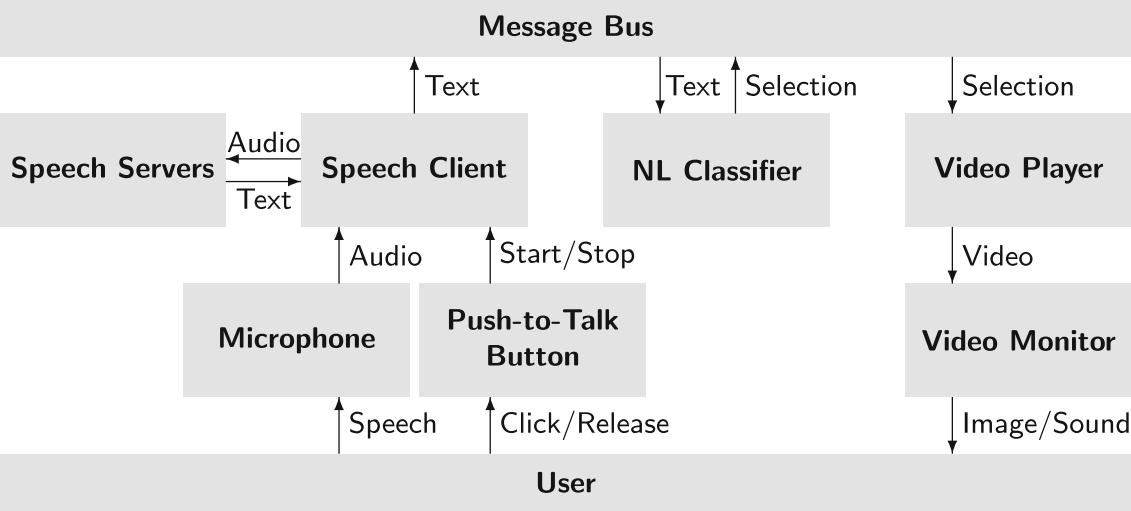
\includegraphics[width=\linewidth*3/4]{TraumDEtAl_DimensionsInTestimony_SystemArchitecture.png}
    \caption{Dimensions in Testimony - Systeem Architectuur \autocite{Traum2015}}
    \label{fig:DiTArchitecture}
\end{figure}

Een ander voorbeeld zijn de home assistenten zoals Google Home, Amazon Echo of Apple HomePod. Zij staan op stand-by tot de gebruiker het triggerwoord zegt, `Hey Google' bijvoorbeeld. Eenmaal geactiveerd luisteren ze naar wat de gebruiker zegt en zetten ze dit aan de hand van een ASR om naar tekst. Daarna haalt het met natuurlijke taalverwerking (NLP) de intentie en sleutelwoorden uit de tekst en genereert daarmee een gepast antwoord. Als laatste zet het gegenereerde tekst om naar spraak.

\subsection{\IfLanguageName{dutch}{Spraakherkening}{Speech recognition}}%

Net als VR is spraakherkenning de laatste jaren veel vooruitgegaan, dit komt omdat er meer data beschikbaar is, de computers sneller en de algoritmes, genaamd deep neural networks, beter zijn. Deze netwerken worden getraind op grote datasets bestaande uit diverse spraakfragmenten. Hieruit leert het de patronen en kenmerken van menselijke spraak. Maar perfect zullen ze nooit zijn zegt \textcite{Hessen2020}. Dit is geen verrassing aangezien zelf mensen vaak nog problemen hebben bij het verstaan van een andere. Er zijn verschillende stappen waar de ASR de fout kan ingaan.

\paragraph{\IfLanguageName{dutch}{Domein problemen}{Domain problems}}%
Onder de domein problemen valt ten eerste galm en geluidshinder. Dit komt voor wanneer een opname gemaakt wordt in een omgeving met veel achtergrond lawaai. Net als mensen heeft de ASR moeilijkheden met het verstaan van de spreker wanneer deze overstemd wordt door de omgeving \autocite{Alharbi2021}. Naast galm en geluidshinder is het ook moeilijker wanneer twee of meer mensen door elkaar spreken. Dit heet spraak overlapping. Een derde domein probleem is domain mismatch. Dit houd in dat er een discrepantie is tussen het domein gebruikt voor het model te trainen en de use case waar het model in wordt gebruikt. Zo zijn bijvoorbeeld nieuwe accenten of andere omgevingen onbekend voor het model. Daarnaast kan het doeleinde een ander jargon bevatten wat lijd tot out-of-vocabulary fouten.

\paragraph{\IfLanguageName{dutch}{Natuurlijke taalverwerking}{Natural language processing}}%
Zoals vermeld in de vorige paragraaf is de use case van groot belang. Taal dat gebruikt wordt verschilt op vele manieren: jongeren gaan andere woorden gebruiken dan hun senioren, iemand in de IT sector gaat een andere woordenschat hebben dan een dokter. Deze verschillen kunnen leiden tot out-of-vocabulary fouten. Dit houd in dat een bepaald model niet getraind is op bepaalde manier van spreken of woordenschat. Een andere oorzaak van OOV is het trainen van een model op een te kleine dataset.

Ook niet iedereen spreekt woorden op dezelfde manier uit. Afhankelijk van de sprekers afkomst zullen ze een bepaalde taal met een bepaald dialect spreken. Ook wanneer ze in een taal anders dan hun moedertaal praten zal er vaak sporen van hun eigen taal herkenbaar blijven. Dit zorgt ervoor dat de uitspraak van een woord niet altijd hetzelfde is.

\paragraph{\IfLanguageName{dutch}{Efficiëntie van apparatuur}{Device efficiency}}%
Als laatste hebben we de gebruikte toestellen. De kwaliteit van de opnameapparatuur kan de nauwkeurigheid van de ASR beïnvloeden. Het gebruik maken van een high-end microfoon tegenover een goedkope kan betere resultaten creëren.


\subsection{\IfLanguageName{dutch}{Begrijpen van natuurlijke taal}{Natural Language Understanding}} \label{ssec:Natural Language Classifier}%

Naast de ASR hebben we ook het begrijpen van natuurlijke taal (NLU). In 'Dimension in Testimony' maakten ze hiervoor gebruik van NCPEditor (Figuur \ref{fig:NPCEArchitecture}). De classifier in dit systeem berekent welke antwoorden op de ingegeven tekst kunnen gegeven worden door de taalmodellen van beide te vergelijken en de antwoorden te rangschikken. Zolang de ingegeven tekst een foutmarge lager dan 50\% blijft, zal het antwoord ongewijzigd blijven \autocite{Leuski2010}.

Een andere bekend taalmodel is GPT-3. Dit model ligt aan de basis van de populaire chatbot ChatGPT.

\begin{figure}[h]
    \centering
    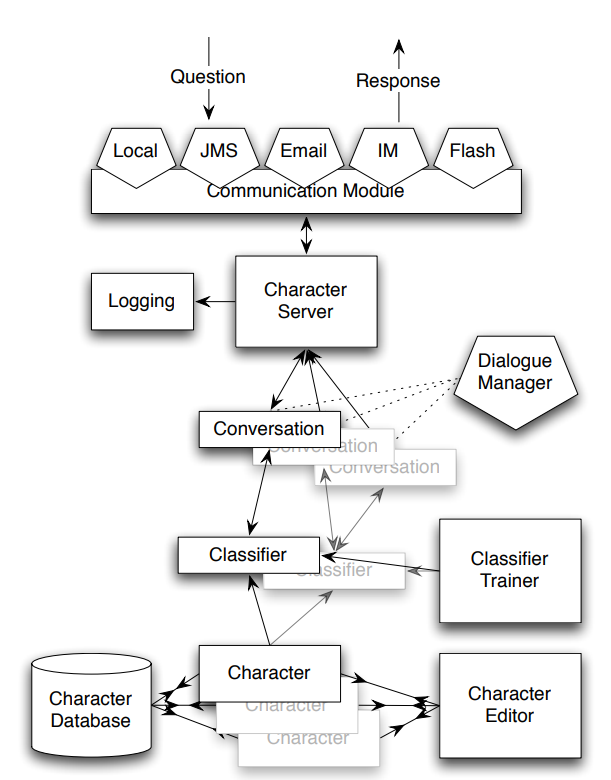
\includegraphics[width=\linewidth*3/4]{Traum&Leuski_NPCEditor_System architecture.png}
    \caption{NPCEditor - Systeem Architectuur \autocite{Leuski2010}}
    \label{fig:NPCEArchitecture}
\end{figure}
